%! TeX program = xelatex
% 如果不需要奇偶面不同的话切换下面两行的注释顺序
% \documentclass[10pt, a4paper, fontset=none, no-math, oneside]{ctexbook}
\documentclass[10pt, a4paper, fontset=none, no-math]{ctexbook}

% % TODO: 增加封面
% TODO: 增加定理盒子

%%%%%%%%%%%%%%%%导入宏包%%%%%%%%%%%%%%%%%%%%


\usepackage[numbers, sort&compress, square]{natbib} % 优化参考文献引用
\usepackage{syntonly} % 编译LaTeX文件后不生成DVI或者PDF文档,只排查错误,要生成文档可以注释\syntaxonly命令
% \syntaxonly
\usepackage{graphicx} % 插入图片
\usepackage{geometry} % 设置页面参数
\usepackage{unicode-math} % 配置 Unicode 数学字体
\usepackage{amsmath} % 用于加载数学公式
% \graphicspath{{figures/}{logo/}} % 用于存放图片的目录figures和logo,这样引用图片的时候就不需要指定目录
\usepackage[x11names]{xcolor} % 用于支持输出颜色
\usepackage{titlesec} % 修改Chapter和Section章节标题的格式
\usepackage{blindtext, lipsum} % 生成英文测试文本
\usepackage{fancyhdr} % 修改页眉页脚的格式
\usepackage{gbt7714} % 参考文献样式
\usepackage{hyperref} % 超链接


%%%%%%%%%%%%%%%%导入宏包%%%%%%%%%%%%%%%%%%%%



%%%%%%%%%%%%%%%%设置字体%%%%%%%%%%%%%%%%%%%%


% 中文字体,具体设置参考ctex宏包
\setCJKmainfont{FZSSJW.TTF}[ % 设置中文主字体为方正书宋 
    Path=./fonts/,
    BoldFont=FZHTJW.TTF, % 设置粗体为方正黑体
    ItalicFont=FZKTJW.TTF, % 设置斜体为方正楷体
]
\setCJKsansfont{FZHTJW.TTF}[Path=./fonts/] % 设置无衬线字体为方正黑体
\setCJKmonofont{FZFSJW.TTF}[Path=./fonts/] % 设置等宽字体为方正仿宋

% 英文字体,具体设置参考fontspec宏包
\setmainfont{CaskaydiaCoveNerdFont}[ % 设置英文主字体为CaskaydiaCove Nerd Font
    Path=./fonts/, % 指定字体文件所在的目录
    Extension=.ttf, % 字体文件后缀
    UprightFont=*-regular, % 正常字体
    BoldFont=*-Bold, % 加粗
    ItalicFont=*-Italic, % 斜体
    BoldItalicFont=*-BoldItalic, % 粗斜体
]
\setsansfont{CaskaydiaCoveNerdFont}[ % 设置英文无衬线字体为CaskaydiaCove Nerd Font
    Path=./fonts/, % 指定字体文件所在的目录
    Extension=.ttf, % 字体文件后缀
    UprightFont=*-regular, % 正常字体
    BoldFont=*-Bold, % 加粗
    ItalicFont=*-Italic, % 斜体
    BoldItalicFont=*-BoldItalic, % 粗斜体
]
\setmonofont{CaskaydiaCoveNerdFontMono}[ % 设置英文等宽字体为CaskaydiaCove Nerd Font Mono
    Path=./fonts/, % 指定字体文件所在的目录
    Extension=.ttf, % 字体文件后缀
    UprightFont=*-regular, % 正常字体
    BoldFont=*-Bold, % 加粗
    ItalicFont=*-Italic, % 斜体
    BoldItalicFont=*-BoldItalic, % 粗斜体
]

% 具体设置参考unicode-math宏包
\setmathfont{TeX Gyre DejaVu Math} % DejaVu风格数学Unicode字体

\linespread{1.25} % 修改行距


%%%%%%%%%%%%%%%%设置字体%%%%%%%%%%%%%%%%%%%%



%%%%%%%%%%%%%%%%页面设置%%%%%%%%%%%%%%%%%%%%


% 具体设置参考geometry宏包
\geometry{
    a4paper,
    inner=1in, % 靠近书脊一侧的边距
    outer=1.25in, % 远离书脊一侧的边距
    top=72pt, % 上边距
    marginparsep=7pt, % 正文区域和边注区域的间距
    marginparwidth=72pt, % 边注区域的宽度
    textheight=700pt, % 正文区域的高度
    footskip=25pt, % 页脚区域和正文区域的间距
}


%%%%%%%%%%%%%%%%页面设置%%%%%%%%%%%%%%%%%%%%



%%%%%%%%%%%%%%%%Chapter设计%%%%%%%%%%%%%%%%%
% 参考:https://stackoverflow.com/questions/78868366/chapter-title-style


% 设置章节编号的字体样式
\newcommand{\chapnumfont}{%     % define font for chapter number
    \usefont{T1}{pnc}{b}{n}%      % choose New Chancery, bold, normal shape
    \fontsize{100}{25}%          % font size 100pt, baselineskip 25pt
    \selectfont%                  % activate font
}
\colorlet{chapnumcol}{red!75!black}  % color for chapter number

% 定义带编号的章节标题样式,具体设置参考titlesec宏包
\titleformat{name=\chapter}[display]
{\filleft\bfseries}
{\filleft\chapnumfont\textcolor{chapnumcol}{\thechapter}}
{0pt}
{\Huge}

% 定义不带编号的章节标题样式,具体设置参考titlesec宏包
\titleformat{name=\chapter,numberless}[display]
{\filright\bfseries}
{\filright}
{0pt}
{\Huge}

% 定义章节和正文等位置的距离,具体设置参考titlesec宏包
\titlespacing{\chapter}{0pt}{0pt}{\baselineskip}


%%%%%%%%%%%%%%%%Chapter设计%%%%%%%%%%%%%%%%%



%%%%%%%%%%%%%%%%Section设计%%%%%%%%%%%%%%%%%
% 如果要在部分标题修改横线的长度可以参考:https://tex.stackexchange.com/questions/299546/length-of-titlerule
% 有关颜色的部分参考xcolor宏包


% 定义带编号的Section样式,具体设置参考titlesec宏包
\titleformat{name=\section}
    {\Large\bfseries}
    {\thesection}
    {1em}
    {}
    % [{\color{DeepPink4}\titlerule[1pt]}]

% 定义带不编号的Section样式,具体设置参考titlesec宏包
\titleformat{name=\section, numberless}
    {\Large\bfseries}
    {}
    {1em}
    {}
    % [{\color{DeepPink4}\titlerule[1pt]}]

% 定义带编号的Subsection样式,具体设置参考titlesec宏包
\titleformat{name=\subsection}
    {\Large\bfseries}
    {\thesubsection}
    {1em}
    {}
    % [{\color{HotPink4}\titlerule[0.8pt]}]

% 定义不带编号的Subsection样式,具体设置参考titlesec宏包
\titleformat{name=\subsection, numberless}
    {\Large\bfseries}
    {}
    {1em}
    {}
    % [{\color{HotPink4}\titlerule[0.8pt]}]


%%%%%%%%%%%%%%%%Section设计%%%%%%%%%%%%%%%%%



%%%%%%%%%%%%%%%页脚页眉设计%%%%%%%%%%%%%%%%%
% 参考:https://tex.stackexchange.com/questions/732462/chapter-number-in-the-header-with-chapter/732464?noredirect=1#comment1824660_732464 


% 详细参数参考fancyhdr宏包
\renewcommand{\chaptermark}[1]{\markboth{\bfseries\uppercase{#1}}{}} % 在双面打印时将章节标题(#1)标记在偶数页的页眉(左边),而奇数页的页眉保持为空。
\renewcommand{\sectionmark}[1]{\markright{\bfseries#1}} % 在单面或双面打印时都将标题(#1)标记在奇数页的页脚(右边)。
\AddToHook {cmd/mainmatter/before} {% 在mainmatter之前重新定义chapter和section的编号格式
    \renewcommand{\chaptermark}[1]{\markboth{\bfseries\uppercase{#1}}{}}%
    \renewcommand{\sectionmark}[1]{\markright{\S \thesection\ \bfseries#1}}%
}
\AddToHook {cmd/backmatter/before} {% 在backmatter之前重新定义chapter和section的编号格式并修改section和chapter的编号
    \renewcommand{\chaptermark}[1]{\markboth{\bfseries\uppercase{#1}}{}}
    \renewcommand{\sectionmark}[1]{\markright{\thesection\ \bfseries#1}}%
    \renewcommand{\thesection}{\Roman{section}}%
}
\pagestyle{fancy} % 设置文档的页面样式为fancy,这意味着页眉和页脚将使用fancyhdr宏包提供的自定义格式。
\fancyhf{} % 清空原本的页脚页眉样式
\fancyhead[RO]{\thepage} % 设置奇数页([RO],即Right, Odd)的页眉右侧(内边)显示的内容为页码(\thepage)。
\fancyhead[LO]{\rightmark}
\fancyhead[LE]{\thepage}
\fancyhead[RE]{\leftmark}
\renewcommand{\headrulewidth}{0.4pt} % 注意不用 \setlength
\renewcommand{\footrulewidth}{0pt} % 去掉页脚的横线


%%%%%%%%%%%%%%%页脚页眉设计%%%%%%%%%%%%%%%%%



%%%%%%%%%%%%%%%参考文献设计%%%%%%%%%%%%%%%%%


\bibliographystyle{gbt7714-numerical} % 顺序编码制


%%%%%%%%%%%%%%%参考文献设计%%%%%%%%%%%%%%%%%



%%%%%%%%%%%%%%%%超链接设计%%%%%%%%%%%%%%%%%%


\hypersetup{
    colorlinks=true, % 启用颜色
    linkcolor=red, % 内部链接的颜色
    citecolor=red, % 引用链接的颜色
    urlcolor=blue!90!black, % 外部链接的颜色
}


%%%%%%%%%%%%%%%%超链接设计%%%%%%%%%%%%%%%%%%


% 导言区,加载宏包和各项设置
%%%%%%%%%%%%%%%%导入宏包%%%%%%%%%%%%%%%%%%%%


\usepackage{ctex}
\usepackage{syntonly} % 编译LaTeX文件后不生成DVI或者PDF文档,只排查错误,要生成文档可以注释\syntaxonly命令
% \syntaxonly
\usepackage{graphicx} % 插入图片
% \graphicspath{{figures/}{logo/}} % 用于存放图片的目录figures和logo,这样引用图片的时候就不需要指定目录


%%%%%%%%%%%%%%%%%%%%%%%%%%%%%%%%%%%%%%%%%%%%



%%%%%%%%%%%%%%%%设置字体%%%%%%%%%%%%%%%%%%%%


% 中文字体,具体设置参考ctex宏包
\setCJKmainfont{FZSSJW.TTF}[ % 设置中文主字体为方正书宋 
    Path=./fonts/,
    BoldFont=FZHTJW.TTF, % 设置粗体为方正黑体
    ItalicFont=FZKTJW.TTF, % 设置斜体为方正楷体
]
\setCJKsansfont{FZHTJW.TTF}[Path=./fonts/] % 设置无衬线字体为方正黑体
\setCJKmonofont{FZFSJW.TTF}[Path=./fonts/] % 设置等宽字体为方正仿宋

% 英文字体,具体设置参考fontspec宏包
\setmainfont{CaskaydiaCoveNerdFont}[ % 设置英文主字体为CaskaydiaCove Nerd Font
    Path=./fonts/, % 指定字体文件所在的目录
    Extension=.ttf, % 字体文件后缀
    UprightFont=*-regular, % 正常字体
    BoldFont=*-Bold, % 加粗
    ItalicFont=*-Italic, % 斜体
    BoldItalicFont=*-BoldItalic]
\setsansfont{CaskaydiaCoveNerdFont}[ % 设置英文无衬线字体为CaskaydiaCove Nerd Font
    Path=./fonts/, % 指定字体文件所在的目录
    Extension=.ttf, % 字体文件后缀
    UprightFont=*-regular, % 正常字体
    BoldFont=*-Bold, % 加粗
    ItalicFont=*-Italic, % 斜体
    BoldItalicFont=*-BoldItalic]
\setmonofont{CaskaydiaCoveNerdFontMono}[ % 设置英文等宽字体为CaskaydiaCove Nerd Font Mono
    Path=./fonts/, % 指定字体文件所在的目录
    Extension=.ttf, % 字体文件后缀
    UprightFont=*-regular, % 正常字体
    BoldFont=*-Bold, % 加粗
    ItalicFont=*-Italic, % 斜体
    BoldItalicFont=*-BoldItalic]


%%%%%%%%%%%%%%%%设置字体%%%%%%%%%%%%%%%%%%%%




\begin{document}

\frontmatter

\chapter{Frontmatter}
\lipsum[5-10]

\mainmatter

\chapter{Introduction}
``你好世界''
这是一段正文的中文文本。
这是一段正文的中文文本。\footnote{Test footnote.}
这是一段正文的中文文本。
这是一段正文的中文文本。

这是一段正文的中文文本。

{\small 这是一段小字的中文文本}

{\Large 这是一段大字的中文文本}

{\itshape 这是一段斜体的中文文本}

\textbf{这是一段加粗正文的中文文本。}\marginpar{这是一段用于边注测试的文本。}

\section{Test 1}

{\CJKfamily{zhmono}
这是一段等宽字体的中文文本。
\textbf{这是一段加粗的等宽字体的中文文本。}
}

{\CJKfamily{zhsans}
这是一段中文无衬线字体的文本。
\textbf{这是一段加粗的中文无衬线字体的文本。}
}

\section{Test 2}

This is a sample text in the main font. \marginpar{Hello, this is a test margin paragraph.}

\textbf{This is a sample bold text in the main font.}

{\sffamily This is a sample text in the sans font.}

{\ttfamily This is a sample text in the mono font.}

\begin{equation}
    \sum_{k=1}^n k^2 = \frac{1}{2} n (n+1)
\end{equation}

\section{Test 3}

\lipsum[30-50]


\chapter{导言}

\lipsum[10-20]

\chapter{Column Generation}

\lipsum[5-10]

\section{Test Column}

\lipsum[10-20]

\backmatter

\chapter*{Appendix}
% \markboth{Appebdix}{Appendix}
\chaptermark{Appendix}

\lipsum[40-50]

\section*{你好,世界!}
% \section*{Hello World}
% \sectionmark{Hello World}
\sectionmark{你好,世界!}

\lipsum[5-10]

\section{Test 4}

\lipsum[10-20]


% \setchapterabstract{This chapter is a foundational concept in probability theory that allows us to assess the likelihood of one event occurring given that another event has already happened. This chapter delves into the key principles and applications of conditional probability. We begin by exploring the fundamental difference between ordinary probability and conditional probability, emphasizing the importance of contextual dependence.}
\chapter{Conditional Probability}
\vspace{-1.5cm}




%%%%%%INSERT TOC BELOW 1ST SECTION%%%%%%%%%%%%

{\chaptoc\noindent\begin{minipage}[inner sep=0,outer sep=0]{0.9\linewidth}\section{Conditional Probability}\end{minipage}}


In our previous lecture, we explored the fundamental concepts of probability theory. We established the core axioms that govern probabilities and their applications in calculating the likelihood of events. However, the world around us is rarely as simple as independent events happening in isolation. Often, the likelihood of one event occurring is influenced by the knowledge of another event having already happened

\Example{Consider a sample space that includes three disjoint events, $A$, $B$, and $C$, as illustrated in Figure \cref{fig:condprobsimp}. Suppose we receive new information confirming that event $A$ has indeed occurred, but we do not have any updates about events $B$ and $C$. How does this additional information about event $A$ affect our original probability model?
}

Since events $A$, $B$, and $C$ are disjoint (as shown\sn{\begin{center}
    

\tikzset{every picture/.style={line width=0.75pt}} %set default line width to 0.75pt        

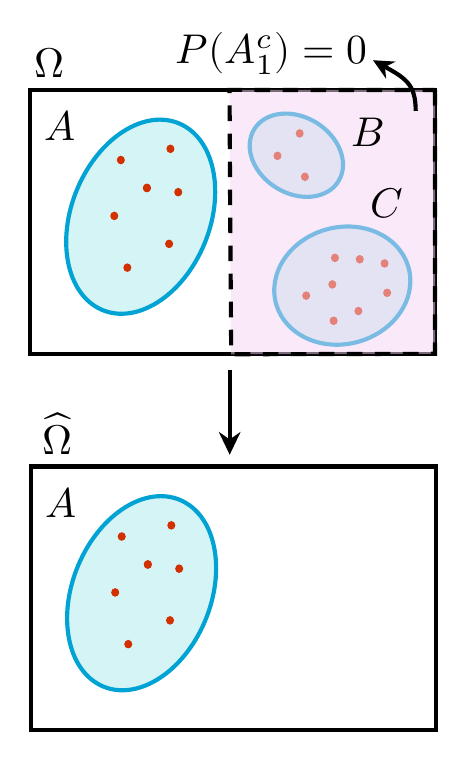
\begin{tikzpicture}[x=0.75pt,y=0.75pt,yscale=-1,xscale=1]
%uncomment if require: \path (0,452); %set diagram left start at 0, and has height of 452

%Shape: Rectangle [id:dp3366248195371335] 
\draw  [color={rgb, 255:red, 0; green, 0; blue, 0 }  ,draw opacity=1 ][line width=1.5]  (8.67,44.29) -- (203.94,44.29) -- (203.94,171.39) -- (8.67,171.39) -- cycle ;
%Shape: Ellipse [id:dp6862156891277029] 
\draw  [color={rgb, 255:red, 0; green, 163; blue, 211 }  ,draw opacity=1 ][fill={rgb, 255:red, 212; green, 244; blue, 245 }  ,fill opacity=1 ][line width=1.5]  (32.57,89.66) .. controls (43.83,65.33) and (66.18,52.63) .. (82.5,61.29) .. controls (98.82,69.95) and (102.92,96.69) .. (91.67,121.02) .. controls (80.41,145.34) and (58.06,158.04) .. (41.74,149.39) .. controls (25.42,140.73) and (21.32,113.99) .. (32.57,89.66) -- cycle ;
%Shape: Ellipse [id:dp4867640161432012] 
\draw  [color={rgb, 255:red, 0; green, 163; blue, 211 }  ,draw opacity=1 ][fill={rgb, 255:red, 212; green, 244; blue, 245 }  ,fill opacity=1 ][line width=1.5]  (126.82,144.95) .. controls (124.18,129.63) and (136.55,114.33) .. (154.46,110.79) .. controls (172.37,107.25) and (189.03,116.8) .. (191.68,132.12) .. controls (194.32,147.44) and (181.95,162.74) .. (164.04,166.28) .. controls (146.13,169.82) and (129.46,160.27) .. (126.82,144.95) -- cycle ;
%Shape: Ellipse [id:dp4008297574108268] 
\draw  [color={rgb, 255:red, 0; green, 163; blue, 211 }  ,draw opacity=1 ][fill={rgb, 255:red, 212; green, 244; blue, 245 }  ,fill opacity=1 ][line width=1.5]  (115.94,64.86) .. controls (120.1,55.54) and (132.96,52.84) .. (144.66,58.84) .. controls (156.36,64.84) and (162.46,77.25) .. (158.3,86.57) .. controls (154.13,95.9) and (141.27,98.59) .. (129.58,92.59) .. controls (117.88,86.6) and (111.77,74.18) .. (115.94,64.86) -- cycle ;
%Shape: Ellipse [id:dp4111178457958402] 
\draw  [color={rgb, 255:red, 211; green, 48; blue, 0 }  ,draw opacity=1 ][fill={rgb, 255:red, 211; green, 48; blue, 0 }  ,fill opacity=1 ] (50.89,78.02) .. controls (50.89,77.04) and (51.63,76.25) .. (52.54,76.25) .. controls (53.46,76.25) and (54.2,77.04) .. (54.2,78.02) .. controls (54.2,78.99) and (53.46,79.79) .. (52.54,79.79) .. controls (51.63,79.79) and (50.89,78.99) .. (50.89,78.02) -- cycle ;
%Shape: Ellipse [id:dp8938370847340988] 
\draw  [color={rgb, 255:red, 211; green, 48; blue, 0 }  ,draw opacity=1 ][fill={rgb, 255:red, 211; green, 48; blue, 0 }  ,fill opacity=1 ] (63.47,91.49) .. controls (63.47,90.51) and (64.21,89.72) .. (65.12,89.72) .. controls (66.04,89.72) and (66.78,90.51) .. (66.78,91.49) .. controls (66.78,92.47) and (66.04,93.26) .. (65.12,93.26) .. controls (64.21,93.26) and (63.47,92.47) .. (63.47,91.49) -- cycle ;
%Shape: Ellipse [id:dp5056604205732773] 
\draw  [color={rgb, 255:red, 211; green, 48; blue, 0 }  ,draw opacity=1 ][fill={rgb, 255:red, 211; green, 48; blue, 0 }  ,fill opacity=1 ] (63.47,91.49) .. controls (63.47,90.51) and (64.21,89.72) .. (65.12,89.72) .. controls (66.04,89.72) and (66.78,90.51) .. (66.78,91.49) .. controls (66.78,92.47) and (66.04,93.26) .. (65.12,93.26) .. controls (64.21,93.26) and (63.47,92.47) .. (63.47,91.49) -- cycle ;
%Shape: Ellipse [id:dp33084323307117347] 
\draw  [color={rgb, 255:red, 211; green, 48; blue, 0 }  ,draw opacity=1 ][fill={rgb, 255:red, 211; green, 48; blue, 0 }  ,fill opacity=1 ] (47.74,104.96) .. controls (47.74,103.98) and (48.48,103.19) .. (49.4,103.19) .. controls (50.31,103.19) and (51.05,103.98) .. (51.05,104.96) .. controls (51.05,105.94) and (50.31,106.73) .. (49.4,106.73) .. controls (48.48,106.73) and (47.74,105.94) .. (47.74,104.96) -- cycle ;
%Shape: Ellipse [id:dp2671439133759155] 
\draw  [color={rgb, 255:red, 211; green, 48; blue, 0 }  ,draw opacity=1 ][fill={rgb, 255:red, 211; green, 48; blue, 0 }  ,fill opacity=1 ] (74.16,118.43) .. controls (74.16,117.46) and (74.9,116.66) .. (75.82,116.66) .. controls (76.73,116.66) and (77.47,117.46) .. (77.47,118.43) .. controls (77.47,119.41) and (76.73,120.2) .. (75.82,120.2) .. controls (74.9,120.2) and (74.16,119.41) .. (74.16,118.43) -- cycle ;
%Shape: Ellipse [id:dp3276259019311121] 
\draw  [color={rgb, 255:red, 211; green, 48; blue, 0 }  ,draw opacity=1 ][fill={rgb, 255:red, 211; green, 48; blue, 0 }  ,fill opacity=1 ] (54.04,129.88) .. controls (54.04,128.91) and (54.78,128.12) .. (55.69,128.12) .. controls (56.6,128.12) and (57.34,128.91) .. (57.34,129.88) .. controls (57.34,130.86) and (56.6,131.65) .. (55.69,131.65) .. controls (54.78,131.65) and (54.04,130.86) .. (54.04,129.88) -- cycle ;
%Shape: Ellipse [id:dp47214739741034384] 
\draw  [color={rgb, 255:red, 211; green, 48; blue, 0 }  ,draw opacity=1 ][fill={rgb, 255:red, 211; green, 48; blue, 0 }  ,fill opacity=1 ] (78.57,93.51) .. controls (78.57,92.53) and (79.31,91.74) .. (80.22,91.74) .. controls (81.13,91.74) and (81.87,92.53) .. (81.87,93.51) .. controls (81.87,94.49) and (81.13,95.28) .. (80.22,95.28) .. controls (79.31,95.28) and (78.57,94.49) .. (78.57,93.51) -- cycle ;
%Shape: Ellipse [id:dp8767298215255175] 
\draw  [color={rgb, 255:red, 211; green, 48; blue, 0 }  ,draw opacity=1 ][fill={rgb, 255:red, 211; green, 48; blue, 0 }  ,fill opacity=1 ] (74.79,72.63) .. controls (74.79,71.65) and (75.53,70.86) .. (76.45,70.86) .. controls (77.36,70.86) and (78.1,71.65) .. (78.1,72.63) .. controls (78.1,73.61) and (77.36,74.4) .. (76.45,74.4) .. controls (75.53,74.4) and (74.79,73.61) .. (74.79,72.63) -- cycle ;
%Shape: Ellipse [id:dp3692224948516316] 
\draw  [color={rgb, 255:red, 211; green, 48; blue, 0 }  ,draw opacity=1 ][fill={rgb, 255:red, 211; green, 48; blue, 0 }  ,fill opacity=1 ] (126.37,76) .. controls (126.37,75.02) and (127.11,74.23) .. (128.03,74.23) .. controls (128.94,74.23) and (129.68,75.02) .. (129.68,76) .. controls (129.68,76.97) and (128.94,77.77) .. (128.03,77.77) .. controls (127.11,77.77) and (126.37,76.97) .. (126.37,76) -- cycle ;
%Shape: Ellipse [id:dp2783265084512472] 
\draw  [color={rgb, 255:red, 211; green, 48; blue, 0 }  ,draw opacity=1 ][fill={rgb, 255:red, 211; green, 48; blue, 0 }  ,fill opacity=1 ] (139.58,86.1) .. controls (139.58,85.12) and (140.32,84.33) .. (141.24,84.33) .. controls (142.15,84.33) and (142.89,85.12) .. (142.89,86.1) .. controls (142.89,87.08) and (142.15,87.87) .. (141.24,87.87) .. controls (140.32,87.87) and (139.58,87.08) .. (139.58,86.1) -- cycle ;
%Shape: Ellipse [id:dp7261549980039332] 
\draw  [color={rgb, 255:red, 211; green, 48; blue, 0 }  ,draw opacity=1 ][fill={rgb, 255:red, 211; green, 48; blue, 0 }  ,fill opacity=1 ] (137.07,65.22) .. controls (137.07,64.24) and (137.81,63.45) .. (138.72,63.45) .. controls (139.63,63.45) and (140.37,64.24) .. (140.37,65.22) .. controls (140.37,66.2) and (139.63,66.99) .. (138.72,66.99) .. controls (137.81,66.99) and (137.07,66.2) .. (137.07,65.22) -- cycle ;
%Shape: Ellipse [id:dp9625327628125422] 
\draw  [color={rgb, 255:red, 211; green, 48; blue, 0 }  ,draw opacity=1 ][fill={rgb, 255:red, 211; green, 48; blue, 0 }  ,fill opacity=1 ] (154.05,125.17) .. controls (154.05,124.19) and (154.79,123.4) .. (155.71,123.4) .. controls (156.62,123.4) and (157.36,124.19) .. (157.36,125.17) .. controls (157.36,126.15) and (156.62,126.94) .. (155.71,126.94) .. controls (154.79,126.94) and (154.05,126.15) .. (154.05,125.17) -- cycle ;
%Shape: Ellipse [id:dp5185619347277652] 
\draw  [color={rgb, 255:red, 211; green, 48; blue, 0 }  ,draw opacity=1 ][fill={rgb, 255:red, 211; green, 48; blue, 0 }  ,fill opacity=1 ] (140.21,143.36) .. controls (140.21,142.38) and (140.95,141.59) .. (141.87,141.59) .. controls (142.78,141.59) and (143.52,142.38) .. (143.52,143.36) .. controls (143.52,144.33) and (142.78,145.13) .. (141.87,145.13) .. controls (140.95,145.13) and (140.21,144.33) .. (140.21,143.36) -- cycle ;
%Shape: Ellipse [id:dp6604572365676322] 
\draw  [color={rgb, 255:red, 211; green, 48; blue, 0 }  ,draw opacity=1 ][fill={rgb, 255:red, 211; green, 48; blue, 0 }  ,fill opacity=1 ] (153.42,155.48) .. controls (153.42,154.5) and (154.16,153.71) .. (155.08,153.71) .. controls (155.99,153.71) and (156.73,154.5) .. (156.73,155.48) .. controls (156.73,156.46) and (155.99,157.25) .. (155.08,157.25) .. controls (154.16,157.25) and (153.42,156.46) .. (153.42,155.48) -- cycle ;
%Shape: Ellipse [id:dp7003243708088849] 
\draw  [color={rgb, 255:red, 211; green, 48; blue, 0 }  ,draw opacity=1 ][fill={rgb, 255:red, 211; green, 48; blue, 0 }  ,fill opacity=1 ] (152.79,137.97) .. controls (152.79,136.99) and (153.53,136.2) .. (154.45,136.2) .. controls (155.36,136.2) and (156.1,136.99) .. (156.1,137.97) .. controls (156.1,138.95) and (155.36,139.74) .. (154.45,139.74) .. controls (153.53,139.74) and (152.79,138.95) .. (152.79,137.97) -- cycle ;
%Shape: Ellipse [id:dp6853825697598586] 
\draw  [color={rgb, 255:red, 211; green, 48; blue, 0 }  ,draw opacity=1 ][fill={rgb, 255:red, 211; green, 48; blue, 0 }  ,fill opacity=1 ] (165.38,150.77) .. controls (165.38,149.79) and (166.12,149) .. (167.03,149) .. controls (167.94,149) and (168.68,149.79) .. (168.68,150.77) .. controls (168.68,151.74) and (167.94,152.54) .. (167.03,152.54) .. controls (166.12,152.54) and (165.38,151.74) .. (165.38,150.77) -- cycle ;
%Shape: Ellipse [id:dp27452318113210206] 
\draw  [color={rgb, 255:red, 211; green, 48; blue, 0 }  ,draw opacity=1 ][fill={rgb, 255:red, 211; green, 48; blue, 0 }  ,fill opacity=1 ] (177.96,127.86) .. controls (177.96,126.89) and (178.7,126.09) .. (179.61,126.09) .. controls (180.52,126.09) and (181.26,126.89) .. (181.26,127.86) .. controls (181.26,128.84) and (180.52,129.63) .. (179.61,129.63) .. controls (178.7,129.63) and (177.96,128.84) .. (177.96,127.86) -- cycle ;
%Shape: Ellipse [id:dp9495623233468491] 
\draw  [color={rgb, 255:red, 211; green, 48; blue, 0 }  ,draw opacity=1 ][fill={rgb, 255:red, 211; green, 48; blue, 0 }  ,fill opacity=1 ] (179.21,142.01) .. controls (179.21,141.03) and (179.95,140.24) .. (180.87,140.24) .. controls (181.78,140.24) and (182.52,141.03) .. (182.52,142.01) .. controls (182.52,142.99) and (181.78,143.78) .. (180.87,143.78) .. controls (179.95,143.78) and (179.21,142.99) .. (179.21,142.01) -- cycle ;
%Shape: Ellipse [id:dp7131942528105673] 
\draw  [color={rgb, 255:red, 211; green, 48; blue, 0 }  ,draw opacity=1 ][fill={rgb, 255:red, 211; green, 48; blue, 0 }  ,fill opacity=1 ] (166,125.84) .. controls (166,124.87) and (166.74,124.07) .. (167.66,124.07) .. controls (168.57,124.07) and (169.31,124.87) .. (169.31,125.84) .. controls (169.31,126.82) and (168.57,127.61) .. (167.66,127.61) .. controls (166.74,127.61) and (166,126.82) .. (166,125.84) -- cycle ;
%Shape: Polygon [id:ds6881418851533576] 
\draw  [fill={rgb, 255:red, 245; green, 212; blue, 244 }  ,fill opacity=0.5 ][dash pattern={on 5.63pt off 4.5pt}][line width=1.5]  (203.94,44.29) -- (203.94,171.39) -- (105.73,171.61) -- (105.2,97.68) -- (104.93,44.25) -- cycle ;
%Curve Lines [id:da042269024046658554] 
\draw [line width=1.5]    (194.62,54.39) .. controls (194.59,40.95) and (189.45,38.37) .. (177.36,31.77) ;
\draw [shift={(174.05,29.95)}, rotate = 29.13] [fill={rgb, 255:red, 0; green, 0; blue, 0 }  ][line width=0.08]  [draw opacity=0] (9.91,-4.76) -- (0,0) -- (9.91,4.76) -- (6.58,0) -- cycle    ;
%Straight Lines [id:da04618455972416813] 
\draw [line width=1.5]    (105,179) -- (105,216) ;
\draw [shift={(105,220)}, rotate = 270] [fill={rgb, 255:red, 0; green, 0; blue, 0 }  ][line width=0.08]  [draw opacity=0] (11.07,-5.32) -- (0,0) -- (11.07,5.32) -- (7.35,0) -- cycle    ;
%Shape: Rectangle [id:dp6211196777653878] 
\draw  [color={rgb, 255:red, 0; green, 0; blue, 0 }  ,draw opacity=1 ][line width=1.5]  (9.11,225.69) -- (204.38,225.69) -- (204.38,352.79) -- (9.11,352.79) -- cycle ;
%Shape: Ellipse [id:dp8000435370413392] 
\draw  [color={rgb, 255:red, 0; green, 163; blue, 211 }  ,draw opacity=1 ][fill={rgb, 255:red, 212; green, 244; blue, 245 }  ,fill opacity=1 ][line width=1.5]  (33.01,271.06) .. controls (44.27,246.73) and (66.62,234.03) .. (82.94,242.69) .. controls (99.26,251.35) and (103.36,278.09) .. (92.11,302.42) .. controls (80.85,326.74) and (58.5,339.44) .. (42.18,330.79) .. controls (25.86,322.13) and (21.76,295.39) .. (33.01,271.06) -- cycle ;
%Shape: Ellipse [id:dp03731012601422612] 
\draw  [color={rgb, 255:red, 211; green, 48; blue, 0 }  ,draw opacity=1 ][fill={rgb, 255:red, 211; green, 48; blue, 0 }  ,fill opacity=1 ] (51.33,259.42) .. controls (51.33,258.44) and (52.07,257.65) .. (52.98,257.65) .. controls (53.9,257.65) and (54.64,258.44) .. (54.64,259.42) .. controls (54.64,260.39) and (53.9,261.19) .. (52.98,261.19) .. controls (52.07,261.19) and (51.33,260.39) .. (51.33,259.42) -- cycle ;
%Shape: Ellipse [id:dp7662796034721766] 
\draw  [color={rgb, 255:red, 211; green, 48; blue, 0 }  ,draw opacity=1 ][fill={rgb, 255:red, 211; green, 48; blue, 0 }  ,fill opacity=1 ] (63.91,272.89) .. controls (63.91,271.91) and (64.65,271.12) .. (65.56,271.12) .. controls (66.48,271.12) and (67.22,271.91) .. (67.22,272.89) .. controls (67.22,273.87) and (66.48,274.66) .. (65.56,274.66) .. controls (64.65,274.66) and (63.91,273.87) .. (63.91,272.89) -- cycle ;
%Shape: Ellipse [id:dp3428571943128822] 
\draw  [color={rgb, 255:red, 211; green, 48; blue, 0 }  ,draw opacity=1 ][fill={rgb, 255:red, 211; green, 48; blue, 0 }  ,fill opacity=1 ] (63.91,272.89) .. controls (63.91,271.91) and (64.65,271.12) .. (65.56,271.12) .. controls (66.48,271.12) and (67.22,271.91) .. (67.22,272.89) .. controls (67.22,273.87) and (66.48,274.66) .. (65.56,274.66) .. controls (64.65,274.66) and (63.91,273.87) .. (63.91,272.89) -- cycle ;
%Shape: Ellipse [id:dp9003120016223698] 
\draw  [color={rgb, 255:red, 211; green, 48; blue, 0 }  ,draw opacity=1 ][fill={rgb, 255:red, 211; green, 48; blue, 0 }  ,fill opacity=1 ] (48.18,286.36) .. controls (48.18,285.38) and (48.92,284.59) .. (49.84,284.59) .. controls (50.75,284.59) and (51.49,285.38) .. (51.49,286.36) .. controls (51.49,287.34) and (50.75,288.13) .. (49.84,288.13) .. controls (48.92,288.13) and (48.18,287.34) .. (48.18,286.36) -- cycle ;
%Shape: Ellipse [id:dp3839640412271208] 
\draw  [color={rgb, 255:red, 211; green, 48; blue, 0 }  ,draw opacity=1 ][fill={rgb, 255:red, 211; green, 48; blue, 0 }  ,fill opacity=1 ] (74.6,299.83) .. controls (74.6,298.86) and (75.34,298.06) .. (76.26,298.06) .. controls (77.17,298.06) and (77.91,298.86) .. (77.91,299.83) .. controls (77.91,300.81) and (77.17,301.6) .. (76.26,301.6) .. controls (75.34,301.6) and (74.6,300.81) .. (74.6,299.83) -- cycle ;
%Shape: Ellipse [id:dp6698541861451095] 
\draw  [color={rgb, 255:red, 211; green, 48; blue, 0 }  ,draw opacity=1 ][fill={rgb, 255:red, 211; green, 48; blue, 0 }  ,fill opacity=1 ] (54.48,311.28) .. controls (54.48,310.31) and (55.22,309.51) .. (56.13,309.51) .. controls (57.04,309.51) and (57.78,310.31) .. (57.78,311.28) .. controls (57.78,312.26) and (57.04,313.05) .. (56.13,313.05) .. controls (55.22,313.05) and (54.48,312.26) .. (54.48,311.28) -- cycle ;
%Shape: Ellipse [id:dp8255589131283008] 
\draw  [color={rgb, 255:red, 211; green, 48; blue, 0 }  ,draw opacity=1 ][fill={rgb, 255:red, 211; green, 48; blue, 0 }  ,fill opacity=1 ] (79.01,274.91) .. controls (79.01,273.93) and (79.75,273.14) .. (80.66,273.14) .. controls (81.57,273.14) and (82.31,273.93) .. (82.31,274.91) .. controls (82.31,275.89) and (81.57,276.68) .. (80.66,276.68) .. controls (79.75,276.68) and (79.01,275.89) .. (79.01,274.91) -- cycle ;
%Shape: Ellipse [id:dp24911848079184118] 
\draw  [color={rgb, 255:red, 211; green, 48; blue, 0 }  ,draw opacity=1 ][fill={rgb, 255:red, 211; green, 48; blue, 0 }  ,fill opacity=1 ] (75.23,254.03) .. controls (75.23,253.05) and (75.97,252.26) .. (76.89,252.26) .. controls (77.8,252.26) and (78.54,253.05) .. (78.54,254.03) .. controls (78.54,255.01) and (77.8,255.8) .. (76.89,255.8) .. controls (75.97,255.8) and (75.23,255.01) .. (75.23,254.03) -- cycle ;

% Text Node
\draw (8.88,22.37) node [anchor=north west][inner sep=0.75pt]  [xscale=1.5,yscale=1.5]  {$\Omega $};
% Text Node
\draw (13.88,52.5) node [anchor=north west][inner sep=0.75pt]  [xscale=1.5,yscale=1.5]  {$A$};
% Text Node
\draw (161.81,56.09) node [anchor=north west][inner sep=0.75pt]  [xscale=1.5,yscale=1.5]  {$B$};
% Text Node
\draw (171.13,89.67) node [anchor=north west][inner sep=0.75pt]  [xscale=1.5,yscale=1.5]  {$C$};
% Text Node
\draw (76.89,14.53) node [anchor=north west][inner sep=0.75pt]  [xscale=1.5,yscale=1.5]  {$\mathds{P}\left(A_{1}^{c}\right)=0$};
% Text Node
\draw (14.32,233.9) node [anchor=north west][inner sep=0.75pt]  [xscale=1.5,yscale=1.5]  {$A$};
% Text Node
\draw (12.93,197.99) node [anchor=north west][inner sep=0.75pt]  [xscale=1.5,yscale=1.5]  {$\widehat{\Omega}$};


\end{tikzpicture}
\end{center}\captionof{figure}{Visual representation of the conditional probability of event $B$ and $C$ given event A. When $A$ occurs, the probability of $B$ and $C$ also occurring is zero, since the three events are mutually exclusive.}\label{fig:condprobsimp}} in Figure \cref{fig:condprobsimp}), they cannot happen at the same time. This means that if event $A$ occurs, events $B$ and $C$ cannot occur. Events $B$ and $C$ together form the complement of event $A$, denoted as $B \cup C = A^{c}$. Therefore, if $A$ is observed, $A^c$ cannot be observed, i.e.
\[
\mathds{P}(A^{c})=\mathds{P}(B \cup C)\overset{\text{(A3)}}{=}\mathds{P}(B) + \mathds{P}(C) = 0
\]
If and only if $\mathds{P}(B)=\mathds{P}(C)=0$.

In this modified sample space, the probability distribution is also updated. The probability of event $A$ occurring is now $1$, which makes it a new sample space by axiom (A2), i.e. $\widehat{\Omega}\triangleq A$ , since it is the only event in the new sample space.

\Example{
Consider a sample space that includes three events, $A$, $B$, and $C$, of which event $C$ is disjoint from events $A$ and $B$, but events $A$ and $B$ are not disjoint as illustrated in Figure \cref{fig:condprobvis}. Suppose we receive new information confirming that event $A$ has indeed occurred, but we do not have any updates about events $B$ and $C$. How does this additional information about event $A$ affect our original probability model?
}

When we confirm that event $A$ has occurred, we must revise our probability model to reflect this new information as done in the previous example. Since event $C$ is mutually exclusive with events $A$ and $B$, we can immediately conclude that event $C$ can not occur, i.e. $\mathds{P}(C)=0$.

Event\sn{\begin{center}
    

\tikzset{every picture/.style={line width=0.75pt}} %set default line width to 0.75pt        

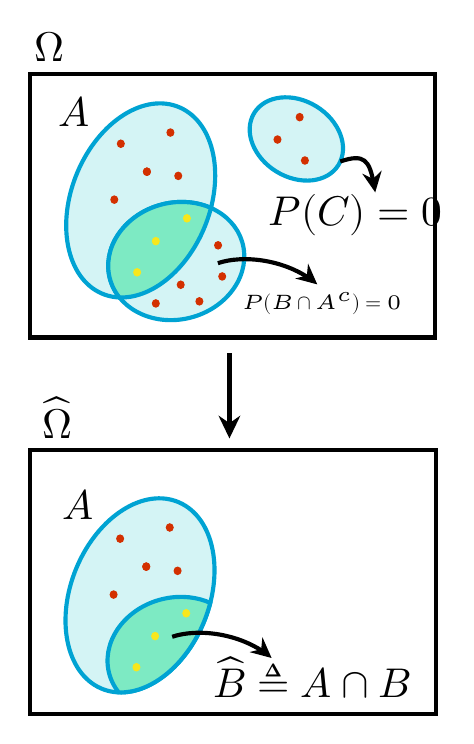
\begin{tikzpicture}[x=0.75pt,y=0.75pt,yscale=-1,xscale=1]
%uncomment if require: \path (0,397); %set diagram left start at 0, and has height of 397

%Straight Lines [id:da04618455972416813] 
\draw [line width=1.5]    (105,179) -- (105,216) ;
\draw [shift={(105,220)}, rotate = 270] [fill={rgb, 255:red, 0; green, 0; blue, 0 }  ][line width=0.08]  [draw opacity=0] (11.07,-5.32) -- (0,0) -- (11.07,5.32) -- (7.35,0) -- cycle    ;
%Shape: Rectangle [id:dp6211196777653878] 
\draw  [color={rgb, 255:red, 0; green, 0; blue, 0 }  ,draw opacity=1 ][line width=1.5]  (9.11,225.69) -- (204.38,225.69) -- (204.38,352.79) -- (9.11,352.79) -- cycle ;
%Shape: Rectangle [id:dp9414156037094199] 
\draw  [color={rgb, 255:red, 0; green, 0; blue, 0 }  ,draw opacity=1 ][line width=1.5]  (8.79,44.29) -- (204.06,44.29) -- (204.06,171.39) -- (8.79,171.39) -- cycle ;
%Shape: Ellipse [id:dp00230890425695085] 
\draw  [color={rgb, 255:red, 0; green, 163; blue, 211 }  ,draw opacity=1 ][fill={rgb, 255:red, 212; green, 244; blue, 245 }  ,fill opacity=1 ][line width=1.5]  (32.69,89.66) .. controls (43.95,65.33) and (66.3,52.63) .. (82.62,61.29) .. controls (98.94,69.95) and (103.04,96.69) .. (91.79,121.02) .. controls (80.53,145.34) and (58.18,158.04) .. (41.86,149.39) .. controls (25.54,140.73) and (21.44,113.99) .. (32.69,89.66) -- cycle ;
%Shape: Ellipse [id:dp5376808010965288] 
\draw  [color={rgb, 255:red, 0; green, 163; blue, 211 }  ,draw opacity=1 ][fill={rgb, 255:red, 212; green, 244; blue, 245 }  ,fill opacity=1 ][line width=1.5]  (46.94,140.95) .. controls (44.3,125.63) and (56.67,110.33) .. (74.58,106.79) .. controls (92.49,103.25) and (109.15,112.8) .. (111.8,128.12) .. controls (114.44,143.44) and (102.07,158.74) .. (84.16,162.28) .. controls (66.25,165.82) and (49.58,156.27) .. (46.94,140.95) -- cycle ;
%Shape: Ellipse [id:dp11813897967702469] 
\draw  [color={rgb, 255:red, 0; green, 163; blue, 211 }  ,draw opacity=1 ][fill={rgb, 255:red, 212; green, 244; blue, 245 }  ,fill opacity=1 ][line width=1.5]  (116.06,64.86) .. controls (120.23,55.54) and (133.08,52.84) .. (144.78,58.84) .. controls (156.48,64.84) and (162.59,77.25) .. (158.42,86.57) .. controls (154.25,95.9) and (141.4,98.59) .. (129.7,92.59) .. controls (118,86.6) and (111.89,74.18) .. (116.06,64.86) -- cycle ;
%Shape: Ellipse [id:dp49451969983731026] 
\draw  [color={rgb, 255:red, 211; green, 48; blue, 0 }  ,draw opacity=1 ][fill={rgb, 255:red, 211; green, 48; blue, 0 }  ,fill opacity=1 ] (51.01,78.02) .. controls (51.01,77.04) and (51.75,76.25) .. (52.66,76.25) .. controls (53.58,76.25) and (54.32,77.04) .. (54.32,78.02) .. controls (54.32,78.99) and (53.58,79.79) .. (52.66,79.79) .. controls (51.75,79.79) and (51.01,78.99) .. (51.01,78.02) -- cycle ;
%Shape: Ellipse [id:dp46303952773358925] 
\draw  [color={rgb, 255:red, 211; green, 48; blue, 0 }  ,draw opacity=1 ][fill={rgb, 255:red, 211; green, 48; blue, 0 }  ,fill opacity=1 ] (63.59,91.49) .. controls (63.59,90.51) and (64.33,89.72) .. (65.24,89.72) .. controls (66.16,89.72) and (66.9,90.51) .. (66.9,91.49) .. controls (66.9,92.47) and (66.16,93.26) .. (65.24,93.26) .. controls (64.33,93.26) and (63.59,92.47) .. (63.59,91.49) -- cycle ;
%Shape: Ellipse [id:dp11111212725661623] 
\draw  [color={rgb, 255:red, 211; green, 48; blue, 0 }  ,draw opacity=1 ][fill={rgb, 255:red, 211; green, 48; blue, 0 }  ,fill opacity=1 ] (63.59,91.49) .. controls (63.59,90.51) and (64.33,89.72) .. (65.24,89.72) .. controls (66.16,89.72) and (66.9,90.51) .. (66.9,91.49) .. controls (66.9,92.47) and (66.16,93.26) .. (65.24,93.26) .. controls (64.33,93.26) and (63.59,92.47) .. (63.59,91.49) -- cycle ;
%Shape: Ellipse [id:dp04173640922649979] 
\draw  [color={rgb, 255:red, 211; green, 48; blue, 0 }  ,draw opacity=1 ][fill={rgb, 255:red, 211; green, 48; blue, 0 }  ,fill opacity=1 ] (47.87,104.96) .. controls (47.87,103.98) and (48.61,103.19) .. (49.52,103.19) .. controls (50.43,103.19) and (51.17,103.98) .. (51.17,104.96) .. controls (51.17,105.94) and (50.43,106.73) .. (49.52,106.73) .. controls (48.61,106.73) and (47.87,105.94) .. (47.87,104.96) -- cycle ;
%Shape: Ellipse [id:dp5634605320521795] 
\draw  [color={rgb, 255:red, 211; green, 48; blue, 0 }  ,draw opacity=1 ][fill={rgb, 255:red, 211; green, 48; blue, 0 }  ,fill opacity=1 ] (74.29,118.43) .. controls (74.29,117.46) and (75.03,116.66) .. (75.94,116.66) .. controls (76.85,116.66) and (77.59,117.46) .. (77.59,118.43) .. controls (77.59,119.41) and (76.85,120.2) .. (75.94,120.2) .. controls (75.03,120.2) and (74.29,119.41) .. (74.29,118.43) -- cycle ;
%Shape: Ellipse [id:dp3326298965670931] 
\draw  [color={rgb, 255:red, 211; green, 48; blue, 0 }  ,draw opacity=1 ][fill={rgb, 255:red, 211; green, 48; blue, 0 }  ,fill opacity=1 ] (54.16,129.88) .. controls (54.16,128.91) and (54.9,128.12) .. (55.81,128.12) .. controls (56.72,128.12) and (57.46,128.91) .. (57.46,129.88) .. controls (57.46,130.86) and (56.72,131.65) .. (55.81,131.65) .. controls (54.9,131.65) and (54.16,130.86) .. (54.16,129.88) -- cycle ;
%Shape: Ellipse [id:dp7660013441945923] 
\draw  [color={rgb, 255:red, 211; green, 48; blue, 0 }  ,draw opacity=1 ][fill={rgb, 255:red, 211; green, 48; blue, 0 }  ,fill opacity=1 ] (78.69,93.51) .. controls (78.69,92.53) and (79.43,91.74) .. (80.34,91.74) .. controls (81.25,91.74) and (81.99,92.53) .. (81.99,93.51) .. controls (81.99,94.49) and (81.25,95.28) .. (80.34,95.28) .. controls (79.43,95.28) and (78.69,94.49) .. (78.69,93.51) -- cycle ;
%Shape: Ellipse [id:dp2640720394663316] 
\draw  [color={rgb, 255:red, 211; green, 48; blue, 0 }  ,draw opacity=1 ][fill={rgb, 255:red, 211; green, 48; blue, 0 }  ,fill opacity=1 ] (74.91,72.63) .. controls (74.91,71.65) and (75.65,70.86) .. (76.57,70.86) .. controls (77.48,70.86) and (78.22,71.65) .. (78.22,72.63) .. controls (78.22,73.61) and (77.48,74.4) .. (76.57,74.4) .. controls (75.65,74.4) and (74.91,73.61) .. (74.91,72.63) -- cycle ;
%Shape: Ellipse [id:dp693934108202442] 
\draw  [color={rgb, 255:red, 211; green, 48; blue, 0 }  ,draw opacity=1 ][fill={rgb, 255:red, 211; green, 48; blue, 0 }  ,fill opacity=1 ] (126.5,76) .. controls (126.5,75.02) and (127.24,74.23) .. (128.15,74.23) .. controls (129.06,74.23) and (129.8,75.02) .. (129.8,76) .. controls (129.8,76.97) and (129.06,77.77) .. (128.15,77.77) .. controls (127.24,77.77) and (126.5,76.97) .. (126.5,76) -- cycle ;
%Shape: Ellipse [id:dp23706410013222534] 
\draw  [color={rgb, 255:red, 211; green, 48; blue, 0 }  ,draw opacity=1 ][fill={rgb, 255:red, 211; green, 48; blue, 0 }  ,fill opacity=1 ] (139.71,86.1) .. controls (139.71,85.12) and (140.45,84.33) .. (141.36,84.33) .. controls (142.27,84.33) and (143.01,85.12) .. (143.01,86.1) .. controls (143.01,87.08) and (142.27,87.87) .. (141.36,87.87) .. controls (140.45,87.87) and (139.71,87.08) .. (139.71,86.1) -- cycle ;
%Shape: Ellipse [id:dp6360572798902322] 
\draw  [color={rgb, 255:red, 211; green, 48; blue, 0 }  ,draw opacity=1 ][fill={rgb, 255:red, 211; green, 48; blue, 0 }  ,fill opacity=1 ] (137.19,65.22) .. controls (137.19,64.24) and (137.93,63.45) .. (138.84,63.45) .. controls (139.76,63.45) and (140.5,64.24) .. (140.5,65.22) .. controls (140.5,66.2) and (139.76,66.99) .. (138.84,66.99) .. controls (137.93,66.99) and (137.19,66.2) .. (137.19,65.22) -- cycle ;
%Shape: Path Data [id:dp7259149736223844] 
\draw  [color={rgb, 255:red, 0; green, 163; blue, 211 }  ,draw opacity=1 ][fill={rgb, 255:red, 125; green, 234; blue, 195 }  ,fill opacity=1 ][line width=1.5]  (91.79,121.02) .. controls (82.73,140.58) and (66.5,152.63) .. (52,152.09) .. controls (49.44,148.91) and (47.66,145.15) .. (46.94,140.95) .. controls (44.3,125.63) and (56.67,110.33) .. (74.58,106.79) .. controls (82.33,105.26) and (89.85,106.18) .. (96.1,108.95) .. controls (95.06,112.98) and (93.63,117.03) .. (91.79,121.02) -- cycle ;
%Shape: Ellipse [id:dp8748029195452189] 
\draw  [color={rgb, 255:red, 248; green, 231; blue, 28 }  ,draw opacity=1 ][fill={rgb, 255:red, 248; green, 231; blue, 28 }  ,fill opacity=1 ] (67.87,124.96) .. controls (67.87,123.98) and (68.61,123.19) .. (69.52,123.19) .. controls (70.43,123.19) and (71.17,123.98) .. (71.17,124.96) .. controls (71.17,125.94) and (70.43,126.73) .. (69.52,126.73) .. controls (68.61,126.73) and (67.87,125.94) .. (67.87,124.96) -- cycle ;
%Shape: Ellipse [id:dp35892107978900323] 
\draw  [color={rgb, 255:red, 248; green, 231; blue, 28 }  ,draw opacity=1 ][fill={rgb, 255:red, 248; green, 231; blue, 28 }  ,fill opacity=1 ] (82.87,113.96) .. controls (82.87,112.98) and (83.61,112.19) .. (84.52,112.19) .. controls (85.43,112.19) and (86.17,112.98) .. (86.17,113.96) .. controls (86.17,114.94) and (85.43,115.73) .. (84.52,115.73) .. controls (83.61,115.73) and (82.87,114.94) .. (82.87,113.96) -- cycle ;
%Shape: Ellipse [id:dp6303441698240393] 
\draw  [color={rgb, 255:red, 248; green, 231; blue, 28 }  ,draw opacity=1 ][fill={rgb, 255:red, 248; green, 231; blue, 28 }  ,fill opacity=1 ] (58.87,139.96) .. controls (58.87,138.98) and (59.61,138.19) .. (60.52,138.19) .. controls (61.43,138.19) and (62.17,138.98) .. (62.17,139.96) .. controls (62.17,140.94) and (61.43,141.73) .. (60.52,141.73) .. controls (59.61,141.73) and (58.87,140.94) .. (58.87,139.96) -- cycle ;
%Shape: Ellipse [id:dp9148451166971325] 
\draw  [color={rgb, 255:red, 211; green, 48; blue, 0 }  ,draw opacity=1 ][fill={rgb, 255:red, 211; green, 48; blue, 0 }  ,fill opacity=1 ] (67.87,154.96) .. controls (67.87,153.98) and (68.61,153.19) .. (69.52,153.19) .. controls (70.43,153.19) and (71.17,153.98) .. (71.17,154.96) .. controls (71.17,155.94) and (70.43,156.73) .. (69.52,156.73) .. controls (68.61,156.73) and (67.87,155.94) .. (67.87,154.96) -- cycle ;
%Shape: Ellipse [id:dp556596966955911] 
\draw  [color={rgb, 255:red, 211; green, 48; blue, 0 }  ,draw opacity=1 ][fill={rgb, 255:red, 211; green, 48; blue, 0 }  ,fill opacity=1 ] (88.87,153.96) .. controls (88.87,152.98) and (89.61,152.19) .. (90.52,152.19) .. controls (91.43,152.19) and (92.17,152.98) .. (92.17,153.96) .. controls (92.17,154.94) and (91.43,155.73) .. (90.52,155.73) .. controls (89.61,155.73) and (88.87,154.94) .. (88.87,153.96) -- cycle ;
%Shape: Ellipse [id:dp9974774844394332] 
\draw  [color={rgb, 255:red, 211; green, 48; blue, 0 }  ,draw opacity=1 ][fill={rgb, 255:red, 211; green, 48; blue, 0 }  ,fill opacity=1 ] (79.87,145.96) .. controls (79.87,144.98) and (80.61,144.19) .. (81.52,144.19) .. controls (82.43,144.19) and (83.17,144.98) .. (83.17,145.96) .. controls (83.17,146.94) and (82.43,147.73) .. (81.52,147.73) .. controls (80.61,147.73) and (79.87,146.94) .. (79.87,145.96) -- cycle ;
%Shape: Ellipse [id:dp9409580835000857] 
\draw  [color={rgb, 255:red, 211; green, 48; blue, 0 }  ,draw opacity=1 ][fill={rgb, 255:red, 211; green, 48; blue, 0 }  ,fill opacity=1 ] (99.87,141.96) .. controls (99.87,140.98) and (100.61,140.19) .. (101.52,140.19) .. controls (102.43,140.19) and (103.17,140.98) .. (103.17,141.96) .. controls (103.17,142.94) and (102.43,143.73) .. (101.52,143.73) .. controls (100.61,143.73) and (99.87,142.94) .. (99.87,141.96) -- cycle ;
%Shape: Ellipse [id:dp5143132862031108] 
\draw  [color={rgb, 255:red, 211; green, 48; blue, 0 }  ,draw opacity=1 ][fill={rgb, 255:red, 211; green, 48; blue, 0 }  ,fill opacity=1 ] (97.87,126.96) .. controls (97.87,125.98) and (98.61,125.19) .. (99.52,125.19) .. controls (100.43,125.19) and (101.17,125.98) .. (101.17,126.96) .. controls (101.17,127.94) and (100.43,128.73) .. (99.52,128.73) .. controls (98.61,128.73) and (97.87,127.94) .. (97.87,126.96) -- cycle ;
%Shape: Ellipse [id:dp11913246108965403] 
\draw  [color={rgb, 255:red, 0; green, 163; blue, 211 }  ,draw opacity=1 ][fill={rgb, 255:red, 212; green, 244; blue, 245 }  ,fill opacity=1 ][line width=1.5]  (32.36,279.94) .. controls (43.62,255.61) and (65.97,242.91) .. (82.29,251.57) .. controls (98.61,260.23) and (102.71,286.97) .. (91.46,311.3) .. controls (80.2,335.62) and (57.85,348.32) .. (41.53,339.67) .. controls (25.21,331.01) and (21.11,304.27) .. (32.36,279.94) -- cycle ;
%Shape: Ellipse [id:dp7174777738730975] 
\draw  [color={rgb, 255:red, 211; green, 48; blue, 0 }  ,draw opacity=1 ][fill={rgb, 255:red, 211; green, 48; blue, 0 }  ,fill opacity=1 ] (50.68,268.3) .. controls (50.68,267.32) and (51.42,266.53) .. (52.33,266.53) .. controls (53.25,266.53) and (53.99,267.32) .. (53.99,268.3) .. controls (53.99,269.27) and (53.25,270.07) .. (52.33,270.07) .. controls (51.42,270.07) and (50.68,269.27) .. (50.68,268.3) -- cycle ;
%Shape: Ellipse [id:dp22667574104423016] 
\draw  [color={rgb, 255:red, 211; green, 48; blue, 0 }  ,draw opacity=1 ][fill={rgb, 255:red, 211; green, 48; blue, 0 }  ,fill opacity=1 ] (63.26,281.77) .. controls (63.26,280.79) and (64,280) .. (64.92,280) .. controls (65.83,280) and (66.57,280.79) .. (66.57,281.77) .. controls (66.57,282.75) and (65.83,283.54) .. (64.92,283.54) .. controls (64,283.54) and (63.26,282.75) .. (63.26,281.77) -- cycle ;
%Shape: Ellipse [id:dp03797453831613207] 
\draw  [color={rgb, 255:red, 211; green, 48; blue, 0 }  ,draw opacity=1 ][fill={rgb, 255:red, 211; green, 48; blue, 0 }  ,fill opacity=1 ] (63.26,281.77) .. controls (63.26,280.79) and (64,280) .. (64.92,280) .. controls (65.83,280) and (66.57,280.79) .. (66.57,281.77) .. controls (66.57,282.75) and (65.83,283.54) .. (64.92,283.54) .. controls (64,283.54) and (63.26,282.75) .. (63.26,281.77) -- cycle ;
%Shape: Ellipse [id:dp9646107877187724] 
\draw  [color={rgb, 255:red, 211; green, 48; blue, 0 }  ,draw opacity=1 ][fill={rgb, 255:red, 211; green, 48; blue, 0 }  ,fill opacity=1 ] (47.54,295.24) .. controls (47.54,294.26) and (48.28,293.47) .. (49.19,293.47) .. controls (50.1,293.47) and (50.84,294.26) .. (50.84,295.24) .. controls (50.84,296.22) and (50.1,297.01) .. (49.19,297.01) .. controls (48.28,297.01) and (47.54,296.22) .. (47.54,295.24) -- cycle ;
%Shape: Ellipse [id:dp12699685981109088] 
\draw  [color={rgb, 255:red, 211; green, 48; blue, 0 }  ,draw opacity=1 ][fill={rgb, 255:red, 211; green, 48; blue, 0 }  ,fill opacity=1 ] (73.96,308.71) .. controls (73.96,307.74) and (74.7,306.94) .. (75.61,306.94) .. controls (76.52,306.94) and (77.26,307.74) .. (77.26,308.71) .. controls (77.26,309.69) and (76.52,310.48) .. (75.61,310.48) .. controls (74.7,310.48) and (73.96,309.69) .. (73.96,308.71) -- cycle ;
%Shape: Ellipse [id:dp09636352157629768] 
\draw  [color={rgb, 255:red, 211; green, 48; blue, 0 }  ,draw opacity=1 ][fill={rgb, 255:red, 211; green, 48; blue, 0 }  ,fill opacity=1 ] (53.83,320.17) .. controls (53.83,319.19) and (54.57,318.4) .. (55.48,318.4) .. controls (56.39,318.4) and (57.13,319.19) .. (57.13,320.17) .. controls (57.13,321.14) and (56.39,321.94) .. (55.48,321.94) .. controls (54.57,321.94) and (53.83,321.14) .. (53.83,320.17) -- cycle ;
%Shape: Ellipse [id:dp3703309776747472] 
\draw  [color={rgb, 255:red, 211; green, 48; blue, 0 }  ,draw opacity=1 ][fill={rgb, 255:red, 211; green, 48; blue, 0 }  ,fill opacity=1 ] (78.36,283.79) .. controls (78.36,282.81) and (79.1,282.02) .. (80.01,282.02) .. controls (80.93,282.02) and (81.67,282.81) .. (81.67,283.79) .. controls (81.67,284.77) and (80.93,285.56) .. (80.01,285.56) .. controls (79.1,285.56) and (78.36,284.77) .. (78.36,283.79) -- cycle ;
%Shape: Ellipse [id:dp8043969327292428] 
\draw  [color={rgb, 255:red, 211; green, 48; blue, 0 }  ,draw opacity=1 ][fill={rgb, 255:red, 211; green, 48; blue, 0 }  ,fill opacity=1 ] (74.59,262.91) .. controls (74.59,261.93) and (75.33,261.14) .. (76.24,261.14) .. controls (77.15,261.14) and (77.89,261.93) .. (77.89,262.91) .. controls (77.89,263.89) and (77.15,264.68) .. (76.24,264.68) .. controls (75.33,264.68) and (74.59,263.89) .. (74.59,262.91) -- cycle ;
%Shape: Path Data [id:dp18209704651842884] 
\draw  [color={rgb, 255:red, 0; green, 163; blue, 211 }  ,draw opacity=1 ][fill={rgb, 255:red, 125; green, 234; blue, 195 }  ,fill opacity=1 ][line width=1.5]  (91.46,311.3) .. controls (82.4,330.86) and (66.17,342.91) .. (51.67,342.37) .. controls (49.11,339.19) and (47.34,335.43) .. (46.61,331.23) .. controls (43.97,315.91) and (56.34,300.61) .. (74.25,297.07) .. controls (82,295.54) and (89.52,296.46) .. (95.77,299.23) .. controls (94.73,303.26) and (93.3,307.31) .. (91.46,311.3) -- cycle ;
%Shape: Ellipse [id:dp2658598010858566] 
\draw  [color={rgb, 255:red, 248; green, 231; blue, 28 }  ,draw opacity=1 ][fill={rgb, 255:red, 248; green, 231; blue, 28 }  ,fill opacity=1 ] (67.54,315.24) .. controls (67.54,314.26) and (68.28,313.47) .. (69.19,313.47) .. controls (70.1,313.47) and (70.84,314.26) .. (70.84,315.24) .. controls (70.84,316.22) and (70.1,317.01) .. (69.19,317.01) .. controls (68.28,317.01) and (67.54,316.22) .. (67.54,315.24) -- cycle ;
%Shape: Ellipse [id:dp6027041603091343] 
\draw  [color={rgb, 255:red, 248; green, 231; blue, 28 }  ,draw opacity=1 ][fill={rgb, 255:red, 248; green, 231; blue, 28 }  ,fill opacity=1 ] (82.54,304.24) .. controls (82.54,303.26) and (83.28,302.47) .. (84.19,302.47) .. controls (85.1,302.47) and (85.84,303.26) .. (85.84,304.24) .. controls (85.84,305.22) and (85.1,306.01) .. (84.19,306.01) .. controls (83.28,306.01) and (82.54,305.22) .. (82.54,304.24) -- cycle ;
%Shape: Ellipse [id:dp48885424592356874] 
\draw  [color={rgb, 255:red, 248; green, 231; blue, 28 }  ,draw opacity=1 ][fill={rgb, 255:red, 248; green, 231; blue, 28 }  ,fill opacity=1 ] (58.54,330.24) .. controls (58.54,329.26) and (59.28,328.47) .. (60.19,328.47) .. controls (61.1,328.47) and (61.84,329.26) .. (61.84,330.24) .. controls (61.84,331.22) and (61.1,332.01) .. (60.19,332.01) .. controls (59.28,332.01) and (58.54,331.22) .. (58.54,330.24) -- cycle ;
%Curve Lines [id:da8530770414600444] 
\draw [line width=1.5]    (158.42,86.57) .. controls (169.97,82.64) and (172.44,85.8) .. (174.6,97.66) ;
\draw [shift={(175.24,101.44)}, rotate = 260.85] [fill={rgb, 255:red, 0; green, 0; blue, 0 }  ][line width=0.08]  [draw opacity=0] (9.91,-4.76) -- (0,0) -- (9.91,4.76) -- (6.58,0) -- cycle    ;
%Curve Lines [id:da9554191414975919] 
\draw [line width=1.5]    (99.42,135.57) .. controls (111.22,131.55) and (130.52,133.6) .. (144.3,143.43) ;
\draw [shift={(147.31,145.78)}, rotate = 220.55] [fill={rgb, 255:red, 0; green, 0; blue, 0 }  ][line width=0.08]  [draw opacity=0] (9.91,-4.76) -- (0,0) -- (9.91,4.76) -- (6.58,0) -- cycle    ;
%Curve Lines [id:da6195367761893151] 
\draw [line width=1.5]    (77.42,315.57) .. controls (89.22,311.55) and (108.52,313.6) .. (122.3,323.43) ;
\draw [shift={(125.31,325.78)}, rotate = 220.55] [fill={rgb, 255:red, 0; green, 0; blue, 0 }  ][line width=0.08]  [draw opacity=0] (9.91,-4.76) -- (0,0) -- (9.91,4.76) -- (6.58,0) -- cycle    ;

% Text Node
\draw (12.93,197.99) node [anchor=north west][inner sep=0.75pt]  [xscale=1.5,yscale=1.5]  {$\widehat{\Omega }$};
% Text Node
\draw (9,22.37) node [anchor=north west][inner sep=0.75pt]  [xscale=1.5,yscale=1.5]  {$\Omega $};
% Text Node
\draw (20.89,53.56) node [anchor=north west][inner sep=0.75pt]  [xscale=1.5,yscale=1.5]  {$A$};
% Text Node
\draw (22.58,242.9) node [anchor=north west][inner sep=0.75pt]  [xscale=1.5,yscale=1.5]  {$A$};
% Text Node
\draw (95.19,323.13) node [anchor=north west][inner sep=0.75pt]  [xscale=1.5,yscale=1.5]  {$\widehat{B} \triangleq A\cap B$};
% Text Node
\draw (122,100.59) node [anchor=north west][inner sep=0.75pt]  [xscale=1.5,yscale=1.5]  {$\mathds{P}(C) =0$};
% Text Node
\draw (109.52,147.78) node [anchor=north west][inner sep=0.75pt]  [xscale=1.5,yscale=1.5]  {{\tiny$\mathds{P}(B\cap A^{c})=0$}};


\end{tikzpicture}
\end{center}\captionof{figure}{Visual representation of the conditional probability of event $B$ given event $A$. When A occurs, the probability of $B$ also occurring is equivalent to the intersection between $A$ and $B$.}\label{fig:condprobvis}}$B$ can be broken down into two parts: the region where $B$ intersects with $A$ (the green region in Figure \cref{fig:condprobvis}), and the region where $B$ is observed without $A$.
\[
B=(A\cap B)\cup (A^{c}\cap B)
\]
However, since event $A$ is assumed to be observed, the latter region is no longer possible, i.e. $\mathds{P}(A^{c}\cap B)=0$. Therefore, the probability of event $B$ is reduced to
\[
\mathds{P}(B) \overset{\text{(A3)}}{=} \mathds{P}(A \cap B) + \mathds{P}(A^c \cap B) = \mathds{P}(A \cap B)
\]
Now, we need to establish the relationship between the probability of event $A$ and the probability of the intersection of events $A$ and $B$, denoted as $A \cap B$. In the revised model, event $A$ becomes the new sample space, and accordingly we denote it by $\widehat{\Omega}$. Moreover, we denote the intersection of events $A$ and $B$ as $\widehat{B}$ in the revised model. The problem is now equivalent to calculating the probability of $\widehat{B}$ within the new sample space $\widehat{\Omega}$. This is nothing more than a classic demonstration of the discrete uniform law:
\[
\begin{array}{ccl}
\dis\frac{|\widehat{B}|}{|\widehat{\Omega}|} & = & \dis\frac{|A \cap B|}{|A|} \\[0.4cm]
& = & \dis\frac{\dis\nicefrac{\dis|A \cap B|}{\dis|\Omega|}}{\dis\nicefrac{\dis|A|}{\dis|\Omega|}} \\[0.4cm]
& = & \dis\frac{\mathds{P}(A \cap B)}{\mathds{P}(A)}
\end{array}
\]
This ratio represents the probability of event $B$ occurring given that event $A$ has occurred. We define this as the conditional probability of $B$ conditioned on $A$.

\Definition{
Let $A,B\subseteq\Omega$, the conditional probability of an event $B$ conditioned on an event $A$ is given by
\[
\mathds{P}(B\mid A)\triangleq\frac{\mathds{P}(A \cap B)}{\mathds{P}(A)}
\]
}{Conditional Probability}


Referring to Figure \ref{fig:condprobvis}, we can observe that $|A\cap B|= 3$ and $|A| = 8$. Using these values, we can calculate the conditional probability of $B$ given $A$ as:
\[
\begin{array}{ccl}
\mathds{P}(B \mid A) &=& \dis\frac{P(A \cap B)}{P(A)} \\[0.4cm]
&=& \dis\frac{|A \cap B|}{|A|}\\[0.4cm]
&=& \dis\frac{3}{8}
\end{array}
\]

\clearpage 
\section{Die Roll Example}
We consider a simple example where we utilize the conditional probability.
\Example{
Consider two four-faced dice. Let $B$ denote the event that one of the two die resulted in a value of $2$, and the other die resulted in a value of at least $2$. Moreover, define $M\triangleq\max(X,Y)$. What is the probability that $M=3$, where one of the dices has an attained value of $2$?
}

In this example, there are 16 possible outcomes, all equally likely. We define event $B$ as 
\[
B \triangleq \{(x, y)\in X\times Y \mid \min(x, y) = 2\}
\]

meaning one die shows a value of 2 and the other shows a value of least a 2. Figure \cref{fig:condprobexdice} illustrates\sn{\pgfplotsset{compat = 1.16}

\begin{tikzpicture}[scale=0.6,every node/.style={scale=2}]
    \begin{axis}[
        colormap = {custom}{color(0)=(nblue!20) color(1)=(nblue!30) color(2)=(nblue!40) color(3)=(nblue!50) color(4)=(nblue!60) color(5)=(nblue!70) color(6)=(nblue!80) color(7)=(nblue!90) color(8)=(nblue)
        },
        xlabel={$X$},
        ylabel={$Y$},
        xtick={1,2,3,4},
        ytick={1,2,3,4},
        xmin=0.5, xmax=4.5,
        ymin=0.5, ymax=4.5,
        axis on top,
        point meta min=2,
        point meta max=8,
        nodes near coords={\pgfmathprintnumber\pgfplotspointmeta},
        nodes near coords align={center},
    ]
        \addplot [
            matrix plot*,
            mesh/cols=4,
            point meta=explicit,
        ] table [meta=C] {
            x y C
            1 1 2
            1 2 3
            1 3 4
            1 4 5
            2 1 3
            2 2 4
            2 3 5
            2 4 6
            3 1 4
            3 2 5
            3 3 6
            3 4 7
            4 1 5
            4 2 6
            4 3 7
            4 4 8
        };
    
    \fill[red,draw=black,thick] (1.5,1.5) rectangle ++(1.5,0.5);
    \fill[yellow,draw=black,thick] (1.5,2.5) rectangle ++(1.5,0.5);
    \fill[red,draw=black,thick] (1.5,3.5) rectangle ++(1.5,0.5);
    \fill[yellow,draw=black,thick] (2.5,1.5) rectangle ++(1.5,0.5);
    \fill[yellow,draw=black,thick] (2.5,1.5) rectangle ++(1.5,0.5);
    \fill[red,draw=black,thick] (3.5,1.5) rectangle ++(1.5,0.5);
    \end{axis}
\end{tikzpicture}\captionof{figure}{The sample space in this problem is reduced upon the occurrence of the event $B$ (highlighted in red).}\label{fig:condprobexdice}} these scenarios, we can see that event $B$ consists of the outcomes 
\[
B=\{(2,2), (2,3), (2,4), (3,2), (4,2)\}
\] 
Now, we want to find the probability that $M=3$ (i.e., the maximum value is 3) given that event $B$ has occurred. Out of the 5 scenarios for event $B$, only 2 of them result in an observation for $M$:
\[
M=\{(2,3), (3,2)\}
\]
Therefore, the conditional probability is calculated as
\[
\mathds{P}(M=3 \mid B) = \frac{2}{5}.
\]

Alternatively, we can directly apply the conditional probability formula to reach this result. In this case, we have:
\[
\mathds{P}(M=3\mid B)=\frac{\mathds{P}((M=3)\cap B)}{\mathds{P}(B)}=\frac{\nicefrac{2}{16}}{\nicefrac{5}{16}}=\frac{2}{5}
\]

\Remark{Conditional probabilities are same as ordinary probabilities, but applied to different situations. Intrinsically speaking, they obey the standard probability axioms.
}

The only crucial difference lies in the consideration of additional information.  Ordinary probability treats all events independently, while conditional probability takes into account the knowledge that another event has already transpired.  This context-dependence allows conditional probability to capture more nuanced relationships between events.


\section{Properties of Conditional Probability}
Conditional probability is a fundamental concept in probability theory that allows us to update our beliefs about the likelihood of events based on new information. In this section, we will expand our knowledge on conditional probabilities by developing some basic properties.

We begin by emphasizing that conditional probability adheres to the same basic principles as ordinary probability, namely the probability axioms.
\Proposition{Conditional probability satisfies the probability axioms.
}
{We shall demonstrate this for each axiom:
\bi
\item[(A1)] $\mathds{P}(A\mid B)\geqslant 0$, since
\[
\mathds{P}(A\mid B)=\frac{\mathds{P}(A\cap B)\geqslant 0}{\mathds{P}(B)>0}\geqslant 0
\]
\item[(A2)] $\mathds{P}(\Omega\mid B)=1$, since
\[
\mathds{P}(\Omega\mid B)=\frac{\mathds{P}(\Omega\cap B)}{\mathds{P}(B)}=\frac{\mathds{P}(B)}{\mathds{P}(B)}=1
\]
\item[(A3)] Assume $A\cap C=\emptyset$, then
\[
\begin{array}{ccl}
\mathds{P}(A\cup C\mid B)&=&\dis\frac{\mathds{P}\big((A\cup C)\cap B\big)}{\mathds{P}(B)} \\[0.4cm]
&=&\dis\frac{\mathds{P}\big((A\cap B)\cup(C\cap B)\big)}{\mathds{P}(B)} \\[0.4cm]
&=&\dis\frac{\mathds{P}(A\cap B)}{\mathds{P}(B)} + \frac{\mathds{P}(C\cap B)}{\mathds{P}(B)} \\[0.4cm]
&=&\dis\mathds{P}(A\mid B)+\mathds{P}(C\mid B)
\end{array}
\]
Note that the pair of $A$ that belongs in $B$ is also disjoint from the part of $C$ that belongs to $B$.
\ei
}
Thus, this ensures that our calculations and interpretations remain consistent within the framework of probability theory.




\end{document}





